% Generated by recon/fig-closure.mjs — do not edit by hand.
\documentclass[tikz,border=3pt]{standalone}
\usepackage{amsmath}
\definecolor{Guidocol}{HTML}{2a78d6}
\definecolor{Pompiliacol}{HTML}{eb6834}
\definecolor{Caponsacchicol}{HTML}{1baf7a}
\begin{document}
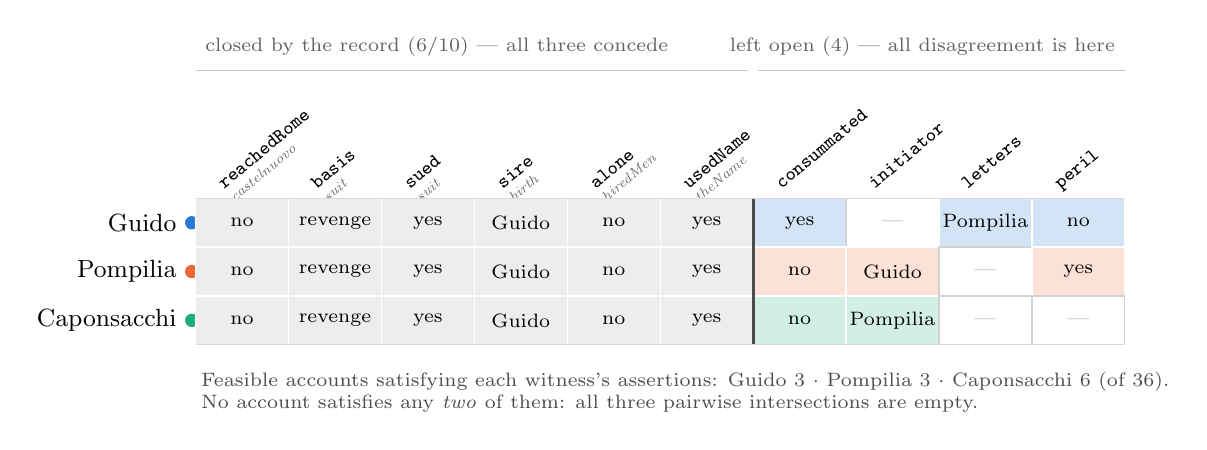
\begin{tikzpicture}[font=\small]

  %% band: who owns which block
  \draw[gray!45, line width=0.5pt] (2.05,1.9300000000000002) -- (9.069999999999999,1.9300000000000002);
  \draw[gray!45, line width=0.5pt] (9.19,1.9300000000000002) -- (13.849999999999998,1.9300000000000002);
  %% anchored to the outer edges, not centred on each block: centring lets the two labels
  %% collide at the divider, which is the one place the figure must stay legible.
  \node[anchor=south west, font=\scriptsize, text=black!62] at (2.05,1.9900000000000002)
    {closed by the record (6/10) --- all three concede};
  \node[anchor=south east, font=\scriptsize, text=black!62] at (13.849999999999998,1.9900000000000002)
    {left open (4) --- all disagreement is here};

  \node[anchor=west, rotate=40, align=left, inner sep=1pt, font=\scriptsize] at (2.3999999999999995,0.372) {\ttfamily reachedRome\\[-2pt]{\tiny\itshape\color{black!58}castelnuovo}};
  \node[anchor=west, rotate=40, align=left, inner sep=1pt, font=\scriptsize] at (3.579999999999999,0.372) {\ttfamily basis\\[-2pt]{\tiny\itshape\color{black!58}suit}};
  \node[anchor=west, rotate=40, align=left, inner sep=1pt, font=\scriptsize] at (4.76,0.372) {\ttfamily sued\\[-2pt]{\tiny\itshape\color{black!58}suit}};
  \node[anchor=west, rotate=40, align=left, inner sep=1pt, font=\scriptsize] at (5.9399999999999995,0.372) {\ttfamily sire\\[-2pt]{\tiny\itshape\color{black!58}birth}};
  \node[anchor=west, rotate=40, align=left, inner sep=1pt, font=\scriptsize] at (7.119999999999999,0.372) {\ttfamily alone\\[-2pt]{\tiny\itshape\color{black!58}hiredMen}};
  \node[anchor=west, rotate=40, align=left, inner sep=1pt, font=\scriptsize] at (8.299999999999999,0.372) {\ttfamily usedName\\[-2pt]{\tiny\itshape\color{black!58}theName}};
  \node[anchor=west, rotate=40, align=left, inner sep=1pt, font=\scriptsize] at (9.479999999999999,0.372) {\ttfamily consummated\\[-2pt]{\tiny\itshape\color{black!58}}};
  \node[anchor=west, rotate=40, align=left, inner sep=1pt, font=\scriptsize] at (10.659999999999998,0.372) {\ttfamily initiator\\[-2pt]{\tiny\itshape\color{black!58}}};
  \node[anchor=west, rotate=40, align=left, inner sep=1pt, font=\scriptsize] at (11.839999999999998,0.372) {\ttfamily letters\\[-2pt]{\tiny\itshape\color{black!58}}};
  \node[anchor=west, rotate=40, align=left, inner sep=1pt, font=\scriptsize] at (13.019999999999998,0.372) {\ttfamily peril\\[-2pt]{\tiny\itshape\color{black!58}}};

  \node[anchor=east, font=\small] at (1.9299999999999997,0) {Guido};
  \node[fill=Guidocol, circle, inner sep=1.7pt] at (1.9999999999999998,0) {};
  \node[anchor=east, font=\small] at (1.9299999999999997,-0.62) {Pompilia};
  \node[fill=Pompiliacol, circle, inner sep=1.7pt] at (1.9999999999999998,-0.62) {};
  \node[anchor=east, font=\small] at (1.9299999999999997,-1.24) {Caponsacchi};
  \node[fill=Caponsacchicol, circle, inner sep=1.7pt] at (1.9999999999999998,-1.24) {};

  \node[draw=white, line width=0.5pt, fill=black!7, minimum width=1.18cm, minimum height=0.62cm, inner sep=0pt, font=\scriptsize] at (2.6399999999999997,0) {no};
  \node[draw=white, line width=0.5pt, fill=black!7, minimum width=1.18cm, minimum height=0.62cm, inner sep=0pt, font=\scriptsize] at (3.8199999999999994,0) {revenge};
  \node[draw=white, line width=0.5pt, fill=black!7, minimum width=1.18cm, minimum height=0.62cm, inner sep=0pt, font=\scriptsize] at (5,0) {yes};
  \node[draw=white, line width=0.5pt, fill=black!7, minimum width=1.18cm, minimum height=0.62cm, inner sep=0pt, font=\scriptsize] at (6.18,0) {Guido};
  \node[draw=white, line width=0.5pt, fill=black!7, minimum width=1.18cm, minimum height=0.62cm, inner sep=0pt, font=\scriptsize] at (7.359999999999999,0) {no};
  \node[draw=white, line width=0.5pt, fill=black!7, minimum width=1.18cm, minimum height=0.62cm, inner sep=0pt, font=\scriptsize] at (8.54,0) {yes};
  \node[draw=white, line width=0.5pt, fill=Guidocol!20, minimum width=1.18cm, minimum height=0.62cm, inner sep=0pt, font=\scriptsize] at (9.719999999999999,0) {yes};
  \node[draw=gray!35, line width=0.5pt, fill=white, minimum width=1.18cm, minimum height=0.62cm, inner sep=0pt, font=\scriptsize] at (10.899999999999999,0) {\textcolor{gray!75}{---}};
  \node[draw=white, line width=0.5pt, fill=Guidocol!20, minimum width=1.18cm, minimum height=0.62cm, inner sep=0pt, font=\scriptsize] at (12.079999999999998,0) {Pompilia};
  \node[draw=white, line width=0.5pt, fill=Guidocol!20, minimum width=1.18cm, minimum height=0.62cm, inner sep=0pt, font=\scriptsize] at (13.259999999999998,0) {no};
  \node[draw=white, line width=0.5pt, fill=black!7, minimum width=1.18cm, minimum height=0.62cm, inner sep=0pt, font=\scriptsize] at (2.6399999999999997,-0.62) {no};
  \node[draw=white, line width=0.5pt, fill=black!7, minimum width=1.18cm, minimum height=0.62cm, inner sep=0pt, font=\scriptsize] at (3.8199999999999994,-0.62) {revenge};
  \node[draw=white, line width=0.5pt, fill=black!7, minimum width=1.18cm, minimum height=0.62cm, inner sep=0pt, font=\scriptsize] at (5,-0.62) {yes};
  \node[draw=white, line width=0.5pt, fill=black!7, minimum width=1.18cm, minimum height=0.62cm, inner sep=0pt, font=\scriptsize] at (6.18,-0.62) {Guido};
  \node[draw=white, line width=0.5pt, fill=black!7, minimum width=1.18cm, minimum height=0.62cm, inner sep=0pt, font=\scriptsize] at (7.359999999999999,-0.62) {no};
  \node[draw=white, line width=0.5pt, fill=black!7, minimum width=1.18cm, minimum height=0.62cm, inner sep=0pt, font=\scriptsize] at (8.54,-0.62) {yes};
  \node[draw=white, line width=0.5pt, fill=Pompiliacol!20, minimum width=1.18cm, minimum height=0.62cm, inner sep=0pt, font=\scriptsize] at (9.719999999999999,-0.62) {no};
  \node[draw=white, line width=0.5pt, fill=Pompiliacol!20, minimum width=1.18cm, minimum height=0.62cm, inner sep=0pt, font=\scriptsize] at (10.899999999999999,-0.62) {Guido};
  \node[draw=gray!35, line width=0.5pt, fill=white, minimum width=1.18cm, minimum height=0.62cm, inner sep=0pt, font=\scriptsize] at (12.079999999999998,-0.62) {\textcolor{gray!75}{---}};
  \node[draw=white, line width=0.5pt, fill=Pompiliacol!20, minimum width=1.18cm, minimum height=0.62cm, inner sep=0pt, font=\scriptsize] at (13.259999999999998,-0.62) {yes};
  \node[draw=white, line width=0.5pt, fill=black!7, minimum width=1.18cm, minimum height=0.62cm, inner sep=0pt, font=\scriptsize] at (2.6399999999999997,-1.24) {no};
  \node[draw=white, line width=0.5pt, fill=black!7, minimum width=1.18cm, minimum height=0.62cm, inner sep=0pt, font=\scriptsize] at (3.8199999999999994,-1.24) {revenge};
  \node[draw=white, line width=0.5pt, fill=black!7, minimum width=1.18cm, minimum height=0.62cm, inner sep=0pt, font=\scriptsize] at (5,-1.24) {yes};
  \node[draw=white, line width=0.5pt, fill=black!7, minimum width=1.18cm, minimum height=0.62cm, inner sep=0pt, font=\scriptsize] at (6.18,-1.24) {Guido};
  \node[draw=white, line width=0.5pt, fill=black!7, minimum width=1.18cm, minimum height=0.62cm, inner sep=0pt, font=\scriptsize] at (7.359999999999999,-1.24) {no};
  \node[draw=white, line width=0.5pt, fill=black!7, minimum width=1.18cm, minimum height=0.62cm, inner sep=0pt, font=\scriptsize] at (8.54,-1.24) {yes};
  \node[draw=white, line width=0.5pt, fill=Caponsacchicol!20, minimum width=1.18cm, minimum height=0.62cm, inner sep=0pt, font=\scriptsize] at (9.719999999999999,-1.24) {no};
  \node[draw=white, line width=0.5pt, fill=Caponsacchicol!20, minimum width=1.18cm, minimum height=0.62cm, inner sep=0pt, font=\scriptsize] at (10.899999999999999,-1.24) {Pompilia};
  \node[draw=gray!35, line width=0.5pt, fill=white, minimum width=1.18cm, minimum height=0.62cm, inner sep=0pt, font=\scriptsize] at (12.079999999999998,-1.24) {\textcolor{gray!75}{---}};
  \node[draw=gray!35, line width=0.5pt, fill=white, minimum width=1.18cm, minimum height=0.62cm, inner sep=0pt, font=\scriptsize] at (13.259999999999998,-1.24) {\textcolor{gray!75}{---}};

  %% the one line that matters: the boundary between what the record settles and what it does not
  \draw[black!70, line width=1.1pt] (9.129999999999999,0.31) -- (9.129999999999999,-1.55);
  \draw[gray!30, line width=0.5pt] (2.05,0.31) -- (13.849999999999998,0.31);
  \draw[gray!30, line width=0.5pt] (2.05,-1.55) -- (13.849999999999998,-1.55);

  \node[anchor=north west, font=\scriptsize, text=black!70, align=left] at (1.9999999999999998,-1.77)
    {Feasible accounts satisfying each witness's assertions: Guido 3 $\cdot$ Pompilia 3 $\cdot$ Caponsacchi 6 (of 36).\\
     No account satisfies any \emph{two} of them: all three pairwise intersections are empty.};

\end{tikzpicture}
\end{document}
